\documentclass[red]{beamer}
\usepackage{etoolbox}
\mode<presentation>

\usetheme{Warsaw}
\usecolortheme{structure} 
\useoutertheme{split}

\makeatletter
\def\th@mystyle{%
    \normalfont % body font
}
\makeatother
\theoremstyle{mystyle}
\newtheorem*{remark}{Remark}
\newtheorem*{ex}{Example}
\newtheorem*{prop}{Proposition}


\usepackage{paralist}
  \let\itemize\compactitem
  \let\enditemize\endcompactitem
  \let\enumerate\compactenum
  \let\endenumerate\endcompactenum
  \let\description\compactdesc
  \let\enddescription\endcompactdesc
  \pltopsep=\medskipamount
  \plitemsep=1pt
  \plparsep=1pt
\usepackage[english]{babel}

%/////////////////////////////////////////////////////////////////////////////
% math pkgs
\usepackage{bbm, bm, amsmath, amssymb, amsthm, mathrsfs, booktabs}

%/////////////////////////////////////////////////////////////////////////////
% tikz
\usepackage{tikz}
\usetikzlibrary{arrows}
\usepackage{poker_slide}


%/////////////////////////////////////////////////////////////////////////////
%/////////////////////////////////////////////////////////////////////////////

\title{Card Shuffling and MCMC Paradigm}
\subtitle{2016 Stochastic Process Course Project}
\author{You Chen, Shu Wang, Ze Yang, Biaojian Feng}
\institute{{advised by}\\ \vspace{.10cm}Prof. Jun Luo}
\date{\scriptsize Antai Collage of Econ \& Mgmt., Shanghai Jiao Tong University\\ \vspace{.10cm}May 8, 2016}


\begin{document}

\frame{
  \titlepage
}

\section{Card Shuffle Problem}
\subsection{Problem Illustration}


\frame
{\frametitle{Illustration of Card Shuffle Problem}
  Given a deck consisting $n$ cards.
  \begin{itemize}
    \item[$\cdot$] The \textbf{sample space} $\Omega:=\{\text{All permutations of the deck.}\}$.
    \item[$\cdot$] The \textbf{cardinality} of sample space: $|\Omega|=n!$
  \end{itemize}
  We want to sample $\omega \in \Omega$, such that every $x$ arises with probability $\mathbb{P}\left(\omega\right)=\frac{1}{n!}$. We want to consider a random variable instead of permutations.
  \begin{definition}[``Index'' of deck permutation]
    Define $X: \Omega \to \mathbb{N}^+$ be the \textbf{lexicographic order} of deck permutation; $X$ is a random variable over $(\Omega, \mathcal{F}, \mathbb{P})$. Moreover, $X\sim \text{Uniform}(\{1,2,..., n!\}).$
  \end{definition}
  \begin{center}
    $X\left(\cards{A}\cards{2}\cards{3}\right)=1$~~~~$X\left(\cards{2}\cards{3}\cards{A}\right)=4$
  \end{center}
}

\frame
{\frametitle{Sampleability of $\text{Uniform}(\{1,2,..., n!\})$}
Sampling a random deck is equivalent to sampling $X$. For a standard deck, $n=52$. How can we sample it?
\begin{itemize}
  \item[(1)] Roll a perfect dice with $52!$ facets.
  \item[$\cdot$] In simulation, ``dice'' is actually a \textbf{random number gernerator (rng)} in computer.
  \item[$\cdot$] The dice provided by GNU C library has at most $2^{31}-1$ facets, which is the largest \textbf{unsigned int} number in 32-bit system. 
  \item[$\cdot$] However, $52!\approx 2^{257}$.
  \item[(2)] Roll 52 independent dices, with $52, 51, 50, ..., 2, 1$ facets respectively.
  \item[(3)] Shuffle, simulate the $52!$ facets' dice.
\end{itemize}
}

\subsection{Shuffling Methods}

\frame
{\frametitle{Modeling Card Shuffle: Shuffling Methods}
  \begin{ex}[Riffle Shuffle] 
  \begin{itemize}
    \item[1.] Split the deck into two parts in each hand.
    \item[2.] Drop the card one after another to merge into new deck, deck card from left hand w.p. $\frac{\text{\# of cards in left hand}}{\text{\# of cards remaining}}$.
  \end{itemize}
  \end{ex}
  \begin{center}
  Input = \cards{A}\cardh{K}\cardc{Q}\cardd{J}\cards{10}\cardh{9}\\
  L: \dcards{A}\cardh{K}\cardc{Q}~~~~R: \cardd{J}\cards{10}\cardh{9} $\xrightarrow{w.p. \frac{1}{2}}$ \cardslot\\
  \end{center}
}

\frame{
  \begin{center}
  L: \dcardh{K}\cardc{Q}~~~~R: \cardd{J}\cards{10}\cardh{9} $\xrightarrow{w.p. \frac{2}{5}}$ \cards{A}\cardslot\\
  L: \cardc{Q}~~~~R: \dcardd{J}\cards{10}\cardh{9} $\xrightarrow{w.p. \frac{3}{4}}$ \cards{A}\cardh{K}\cardslot\\
  L: \dcardc{Q}~~~~R: \cards{10}\cardh{9} $\xrightarrow{w.p. \frac{1}{3}}$ \cards{A}\cardh{K}\cardd{J}\cardslot\\
  \end{center}

  \begin{center}
   Output = \cards{A}\cardh{K}\cardd{J}\cardc{Q}\cards{10}\cardh{9}\\
  \end{center}
}

\frame
{\frametitle{Modeling Card Shuffle: Shuffling Methods}
  \begin{ex}[3-cards Deck Top-in Shuffle] We consider a 3-cards deck shuffled by top-in method. That is, we take one card from the top and insert it at a random position in the deck. If initially, $X_0=X(\{\text{AS, KH, QC}\})=6$
  \end{ex}

  \begin{center}
  \dcards{A}\cardslot\cardh{K}\cardslot\cardc{Q}\cardslot
  \end{center}
  one out of three slots is picked to insert $AS$ with equal probability, hence there are three outcomes w.p. $\frac{1}{3}$
  \begin{center}
    \cards{A}\cardh{K}\cardc{Q}~~~~\cardh{K}\cards{A}\cardc{Q}~~~~\cardh{K}\cardc{Q}\cards{A}
  \end{center}
}

\subsection{Markov Property}

\frame
{
Apply shuffling operation to the initial deck recursively, we obtain a process $\{X_t: t\geq 0\}$. $X_t$ is independent of all history except for $X_{t-1}$. So we can visualize it as a markov process.
\begin{columns}
  \column{0.6\textwidth}
  \newcommand{\markovfig}{
  \begin{center}
  \resizebox{6.8cm}{5.0cm}
  {
    \begin{tikzpicture}[->,>=stealth',shorten >=1pt,auto,node distance=3cm,thick,main node/.style={circle,draw,font=\sffamily\Large\bfseries}]
      \node[main node] (1) {$AKQ(6)$};
      \node[main node] (2) [above right of=1] {$KAQ(4)$};
      \node[main node] (3) [below right of=1] {$KQA(3)$};
      \node[main node] (4) [right of=2] {$QAK(2)$};
      \node[main node] (5) [right of=3] {$QKA(1)$};
      \node[main node] (6) [below right of=4] {$AQK(5)$};

      \path[every node/.style={font=\sffamily\small}]
        (1) edge [bend right=30] node[right]  {} (2)
            edge [left] node[below] {} (3)
            edge [loop left] node[above] {} (1)

        (2) edge [bend right=30] node[above] {} (1)
        edge [bend right=30] node[above] {} (6)
        edge [loop above] node[above] {} (2)

        (3) edge [bend right=30] node[above] {} (4)
        edge [bend right=30] node[below] {} (5)
        edge [loop below] node[below] {} (3)

        (4) edge [bend right=30] node[below] {} (6)
        edge [bend left=30] node[below] {} (1)
        edge [loop above] node[above] {} (4)

        (5) edge [right] node[below] {} (3)
        edge [bend left=30] node[below] {} (2)
        edge [loop below] node[below] {} (5)

        (6) edge [left] node[below] {} (5)
        edge [bend right=30] node[below] {} (4)
        edge [loop right] node[below] {} (6);

        \draw [black] (current bounding box.south west) rectangle (current bounding box.north east);
    \end{tikzpicture}
  }
  \end{center}
  }

  \markovfig

  \column{0.4\textwidth}
  $$\bm{P} = \begin{pmatrix}
    \frac{1}{3} & 0 & \frac{1}{3} & \frac{1}{3} & 0  & 0 \\[5pt]
    0 & \frac{1}{3} & 0 & 0 & \frac{1}{3}  & \frac{1}{3} \\[5pt]
    \frac{1}{3} & \frac{1}{3} & \frac{1}{3} & 0 & 0  & 0 \\[5pt]
    0 & 0 & 0 & \frac{1}{3} & \frac{1}{3}  & \frac{1}{3} \\[5pt]
    \frac{1}{3} & \frac{1}{3} & 0 & 0 & \frac{1}{3}  & 0 \\[5pt]
    0 & 0 & \frac{1}{3} & \frac{1}{3} & 0  & \frac{1}{3} \\
  \end{pmatrix}$$
  \end{columns}
}

\section{The MCMC Paradigm and Related Theory}
\subsection{The MCMC Paradigm}
\frame{
\frametitle{General MCMC Approach}
\textbf{Input}
  \begin{itemize}
    \item[$1$.] a sample space $\Omega$ (may be large or complex).
    \item[$2$.] a positive weight function $w: \Omega \to \mathbb{R}^{+}$.
  \end{itemize}
\textbf{Goal}: 
  We want to draw sample $x\in\Omega$ with some distribution $\pi(x)$ proportional to $w(x)$, i.e.
  $$\pi(x)=\frac{w(x)}{\sum_{x\in \Omega}w(x)}$$
The MCMC algorithm is a general iterative solution to this sampleability problem. We construct a markov chain $\{X_t: t\geq 0\}$, such that $X_t$ converges to our desired sample in (its stationary) distribution. That is:
$$\lim\limits_{t\rightarrow\infty} P^{[t]}(x,y) = \lim\limits_{t\rightarrow\infty}\mathbb{P}\left(X_t=y|X_0=x\right) = \pi(y)$$
}

\frame{
\frametitle{Card Shuffle as MCMC}
\textbf{Input}
  \begin{itemize}
    \item[$1$.] The sample space $\Omega=\{\text{All permutations of the deck.}\}$
    \item[$2$.] We want to sample uniform distribution i.e., $w(k)=1$.
  \end{itemize}
\textbf{Goal}: 
  Draw sample $X\sim \text{Uniform}(\{1,2,...,n!\})$ i.e.
  $$\pi(k)=\frac{w(k)}{\sum_{k\in \Omega}w(k)}=\frac{1}{n!}$$
The constructed markov chain $\{X_t: t\geq 0\}$ is the deck obtained by repeated shuffling. For example, in the 3-cards Deck Top-in Shuffle, we want $1\times 3!$ vector $\bm{\pi}=(\pi(1), \pi(2), ..., \pi(6))$ be the stationary distribution of $\{X_t\}$, i.e.
$$
  \bm{\pi} \bm{P} = \bm{\pi}
$$
}

\subsection{Convergence}
\frame{
\frametitle{Convergence of Markov Chain}
\begin{theorem}[Ergodicity]
If a Markov chain $\{X_t\}$ is irreducible and aperiodic, then it has a unique stationary distribution $\pi(\cdot)$. In particular
\begin{itemize}
  \item[$\cdot$] $\bm{\pi}$ is the unique left eigenvector of $\bm{P}$ corresponding to eigenvalue $\lambda = 1$.
  \item[$\cdot$] $\lim\limits_{t\rightarrow\infty}P^{[t]}(x,y)=\pi(y)$, $\forall x, y\in\Omega$.
\end{itemize}
\end{theorem}

\begin{theorem}[Reversibility]
If Markov chain $\{X_t\}$ is reversible wrt. $\bm{\pi}$, i.e. 
$$\pi(x)P(x,y)=\pi(y)P(y,x)$$
Then $\bm{\pi}$ is the stationary distribution of $\{X_t\}$.
\end{theorem}
}

\frame
{
\begin{remark}
If the probability transition matrix is symmetric: $\bm{P}=\bm{P}^{\top}$, then the markov chain is reversible wrt. uniform distribution. Becasue $\pi(x)=\pi(y)$ and $P(x,y)=P(y,x)$.
\end{remark}

\begin{ex}[3-cards Deck Random Transposition] 
In each iteration, we pick uniformly at random two cards and switch them. We still consider the easy 3-cards deck [AS, KH, QC].
\end{ex}
The first transposition has $\binom{3}{2}=3$ possible outcomes,
\begin{center}
\dcards{A}\dcardh{K}\cardc{Q}~~~~\cards{A}\dcardh{K}\dcardc{Q}~~~~\dcards{A}\cardh{K}\dcardc{Q}\\
\end{center}
}

\frame
{
\begin{center}
  \cardh{K}\cards{A}\cardc{Q}~~~~\cards{A}\cardc{Q}\cardh{K}~~~~\cardc{Q}\cardh{K}\cards{A}
\end{center}
\begin{columns}
\column{0.6\textwidth}
\begin{center}
\resizebox{6.4cm}{4.4cm}
{
\begin{tikzpicture}[<->,>=stealth',shorten >=1pt,auto,node distance=3cm,
                    thick,main node/.style={circle,draw,font=\sffamily\Large\bfseries}]
  \node[main node] (1) {$AKQ(6)$};
  \node[main node] (2) [above right of=1] {$KAQ(4)$};
  \node[main node] (3) [below right of=1] {$KQA(3)$};
  \node[main node] (4) [right of=2] {$QAK(2)$};
  \node[main node] (5) [right of=3] {$QKA(1)$};
  \node[main node] (6) [below right of=4] {$AQK(5)$};


  \path[every node/.style={font=\sffamily\small}]
    (1) edge [right] node[right]  {} (2)
        edge [left] node[below] {} (5)
        edge [left] node[below] {} (6)

    (2) edge [right] node[right]  {} (3)
    edge [right] node[right]  {} (4)

    (3) edge [right] node[right]  {} (6)
    edge [right] node[right]  {} (5)

    (4) edge [right] node[right]  {} (5)
    edge [right] node[right]  {} (6);

  \draw [black] (current bounding box.south west) rectangle (current bounding box.north east);

\end{tikzpicture}
}
\end{center}
\column{0.4\textwidth}
$$\bm{P} = \begin{pmatrix}
  0 & \frac{1}{3} & \frac{1}{3} & 0 & 0  & \frac{1}{3} \\[5pt]
  \frac{1}{3} & 0 & 0 & \frac{1}{3} & \frac{1}{3}  & 0 \\[5pt]
  \frac{1}{3} & 0 & 0 & \frac{1}{3} & \frac{1}{3}  & 0 \\[5pt]
  0 & \frac{1}{3} & \frac{1}{3} & 0 & 0  & \frac{1}{3} \\[5pt]
  0 & \frac{1}{3} & \frac{1}{3} & 0 & 0  & \frac{1}{3} \\[5pt]
  \frac{1}{3} & 0 & 0 & \frac{1}{3} & \frac{1}{3}  & 0 \\
\end{pmatrix}$$
\end{columns}
}

\subsection{Mixing Time}
\frame{\frametitle{Distance Between Distributions}
  We hope to construct a metric to capture how statistically ``close'' two distributional objects are from each other.
  \begin{definition}[Total Variation Norm]
  For two probability mass function $\pi$, $\mu$, define total variation as
  $$\left\|\mu - \pi\right\|_{TV}:=\frac{1}{2}\sum_{x\in \Omega}|\mu(x)-\pi(x)|$$
  In particular, if $\mu(\cdot)=P^{[t]}(x_0,\cdot)$ is conditional distribution of deck $\{X_t\}$, given initial deck $x_0$. $\pi(\cdot)=\frac{1}{n!}$, then we define
  $$\Delta(t):=\left\|P^{[t]}-\pi\right\|_{TV}=\frac{1}{2}\sum_{x\in \Omega}\left|P^{[t]}(x_0, x)-\frac{1}{n!}\right|$$
  \end{definition}

}

\frame{\frametitle{Rate of Convergence}
  \begin{itemize}
    \item[$\cdot$] We apply Monte Carlo simution method, draw large a sample from $P^{[t]}$ (i.e. the deck after $t$ shuffles), then the empirical distribution of sample appoximates $P^{[t]}$.
    \item[$\cdot$] Then, $\Delta(t)$, as a function of $t$, captures the rate by which the Markov chain converges to uniform $\pi(\cdot)$.
    \item[$\cdot$] Moreover, we can set a \textbf{threshold} to $\Delta(t)$ and calculate time needed for the \textbf{deviation of $X_t$ from the limit is bounded by this threshold.}
  \end{itemize}
  \begin{definition}[Mixing Time]
  Set the threshold as constant $s$, the time needed is called Mixing Time of Markov chain associated with threshold $s$, given by
  $$\tau = \min\left\{t: \Delta(t)\leq s\right\}$$
  \end{definition}
}

\section{Simulation Results}

\subsection{Probability Mass Function}

\frame{\frametitle{Mixing of $P^{[t]}$}
\begin{columns}
\column{0.7\textwidth}
  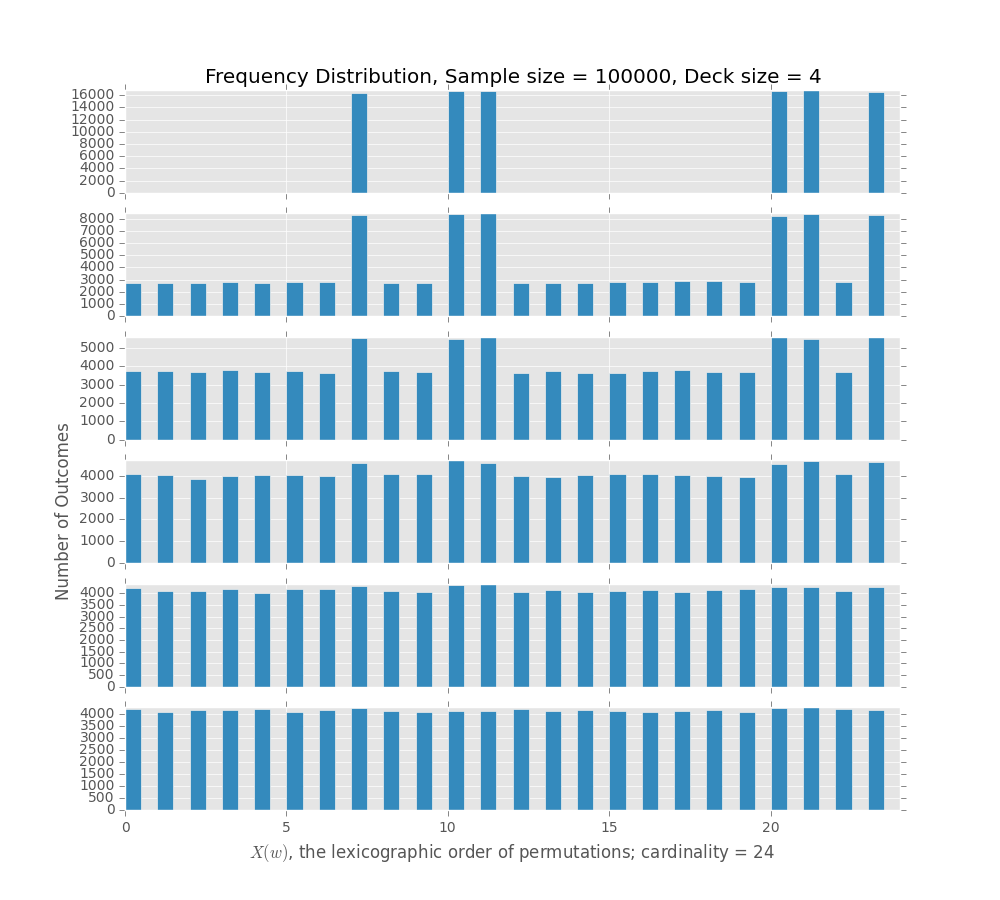
\includegraphics[width=8cm, height=7cm]{figure_2.png}
  \column{0.3\textwidth}
\begin{itemize}
  \item[$\cdot$] Simulation with 4 cards. 
\end{itemize}
\end{columns}
}

\frame{\frametitle{Mixing of $P^{[t]}$}
\begin{columns}
\column{0.7\textwidth}
  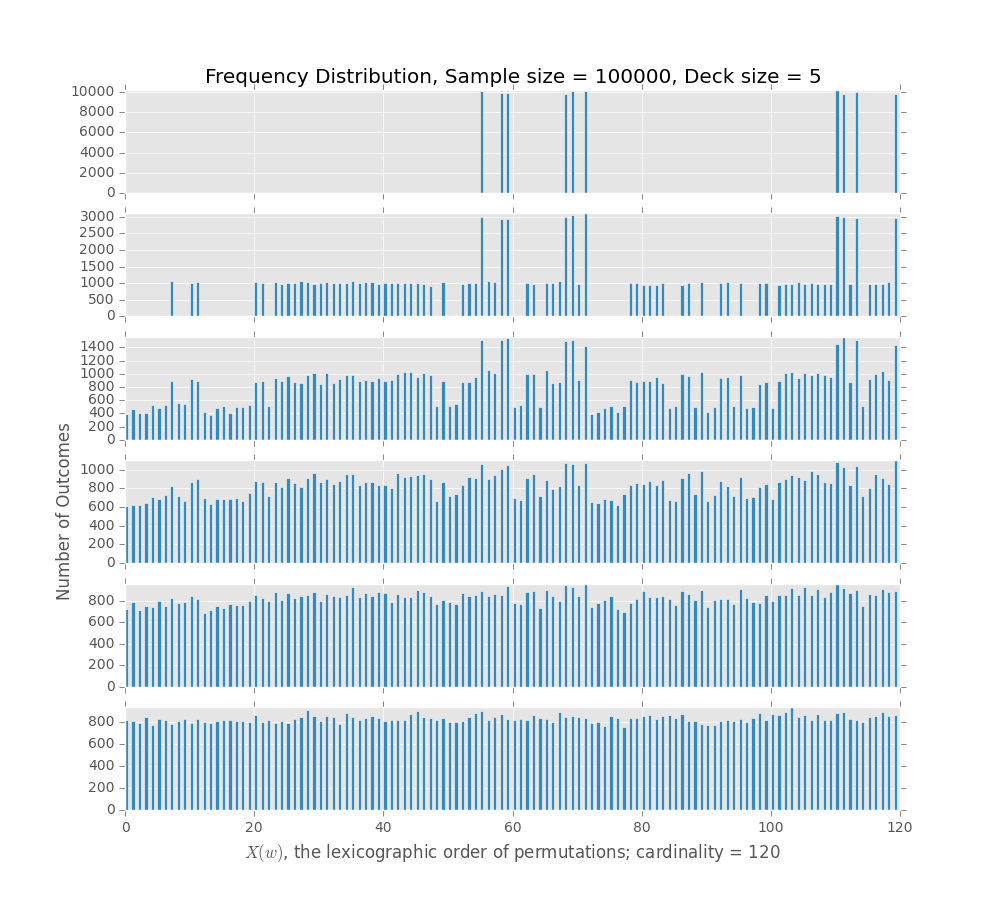
\includegraphics[width=8cm, height=7cm]{figure_3.png}
  \column{0.3\textwidth}
\begin{itemize}
  \item[$\cdot$] Simulation with 5 cards. 
\end{itemize}
\end{columns}
}

\frame{\frametitle{Mixing of $P^{[t]}$: Shuffles in one Plot}
  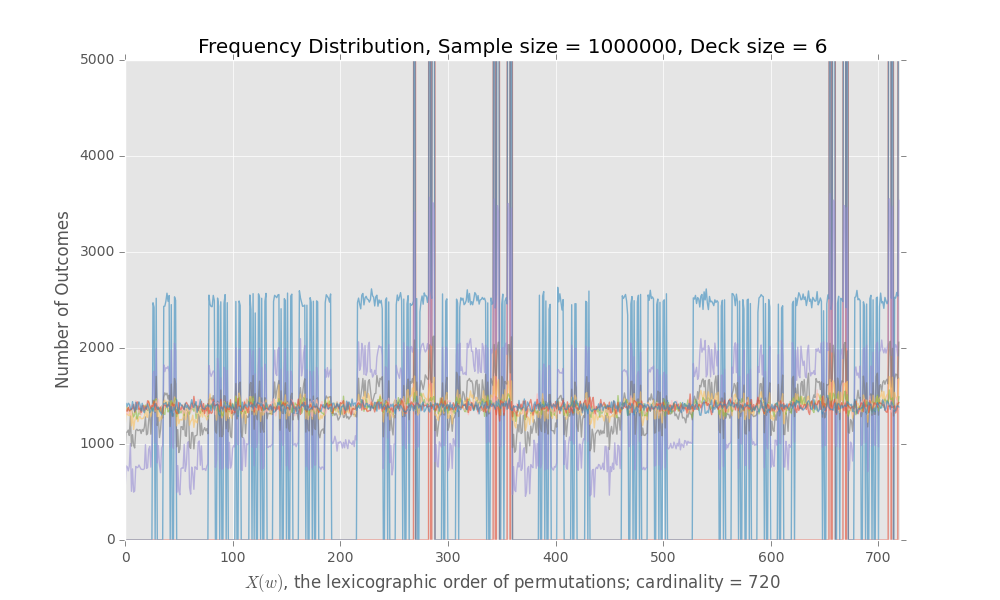
\includegraphics[width=10.5cm, height=6cm]{figure_4.png}
}


\subsection{Total Variation}
\frame{\frametitle{Rate of Convergence}
  \begin{columns}
\column{0.6\textwidth}
  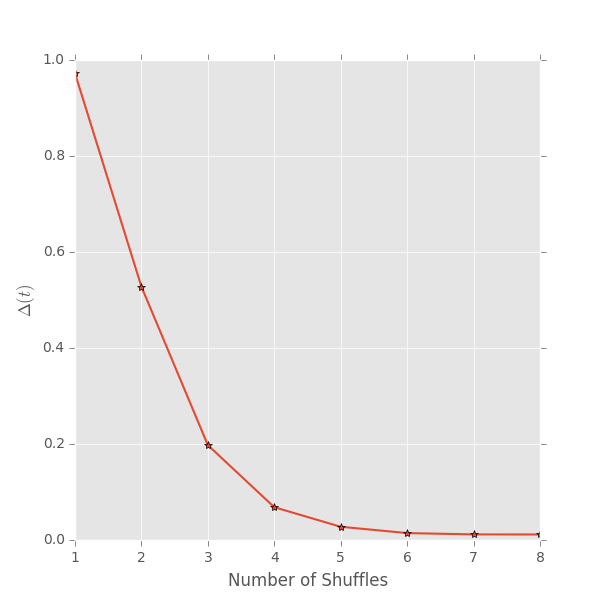
\includegraphics[width=7cm, height=7cm]{figure_5.png}
  \column{0.4\textwidth}
\begin{itemize}
  \item[$\cdot$] (6 cards): $\Delta(7)\approx 0.011$
\end{itemize}
\end{columns}
}

\section*{}
\frame{
\begin{center}
\Huge
  Thanks for your attention.
\end{center}
}


\end{document}